% !TEX root = ../../thesis.tex

\section{Experimental Demonstration of Frequency Regulation \label{sec:exp_building}}
%\begin{abstract}
%Increased penetration of renewable energy sources has increased the demand for frequency regulation reserves.
%In this paper, we demonstrate experimentally that commercial buildings equipped with variable air volume heating ventilation and air conditioning (HVAC) systems can provide frequency regulation. 
%%More specifically, by adjusting the electricity consumption of the supply fans of the HVAC system. 
%A main challenge in this application is that commercial buildings and their HVAC systems are often complex and subject to large disturbances such as occupancy.
%Here, we describe a data-driven method to identify a model that describes the building's thermal dynamics and captures such disturbances.
%In addition, we propose a control scheme that adjusts the electricity consumption of the supply fans of the HVAC system to track the frequency regulation signal, and is suitable for scenarios where an accurate fan model is unavailable. %, e.g. buildings with large uncertainties. 
%We demonstrate the performance of our proposed control scheme through numerous field experiments conducted in an occupied commercial building, and in accordance with PJM's regulation market rules.
%\end{abstract}




%%%%%%%%%%%%%%%%%%%%%%%%%%%%%%%%%%%%%%%%%%%%%%%%%%%%%%%%%%%%%%%
% introduction.tex (part of thesis.tex)
% author: Qie Hu
%
%%%%%%%%%%%%%%%%%%%%%%%%%%%%%%%%%%%%%%%%%%%%%%%%%%%%%%%%%%%%%%%

% !TEX root = ../../thesis.tex


\subsection{Introduction}\label{sec:introduction}

%The operation of a reliable power grid depends on a balance of supply and demand at all times. 
%%Any mismatch can cause the grid frequency to deviate from its nominal value (60 Hz in the U.S.).
%Reserves known as ancillary services (AS) are used to correct any mismatch.
%Amongst them, frequency regulation is the highest quality AS over which the grid operator has almost real-time control and is active continuously during normal operation of the grid, to maintain the grid frequency at its nominal value (60 Hz in the U.S.).
%The recent rapid increase in the penetration of renewable energy sources has increased the volatility and uncertainty of electricity supply, which leads to a greater demand for frequency regulation reserves.
%
%Although these reserves have been traditionally provided by conventional power generators, loads on the demand side have also been considered. 
%%, by increasing (and decreasing) their electricity consumption when the grid frequency increases (decreases).

Commercial buildings are a tremendous untapped resource for frequency regulation provision. 
First, they account for a large fraction of the total electricity consumption (up to 40\% in the U.S., up to 35\% of which is due to heating, ventilation and air conditioning (HVAC) systems \cite{USenergy:2017}). 
Second, the building's large thermal capacity allows the power consumption of HVAC systems be partly shifted in time without compromising occupant comfort. 
Third, many commercial buildings are equipped with a variable frequency drive which can be controlled to vary the power consumption of supply fans of the HVAC system quickly and continuously \cite{Hao:2012demandresponse}. This greatly simplifies tracking of the reference regulation signal, as opposed to resources with on-off control.
%as opposed to on-off control of other equipments such as residential air conditioners and electric vehicles.
Fourth, about one third of commercial buildings in the U.S. are equipped with a building automation system (BAS) \cite{Braun:2012} which facilitates the implementation of new controllers.


On the other hand, there are a number of challenges in using commercial buildings for frequency regulation. 
First, obtaining a building model that is amenable to control is not straightforward. 
Because commercial buildings are often subject to large disturbances such as occupancy, that are difficult to capture. 
%In addition, they have many rooms and the rooms may be affected by different types of disturbances. 
In addition, buildings are often not sufficiently excited, as they must satisfy strict regulatory requirements during regular operation, which limit the type and duration of excitation experiments that can be conducted.
Second, about one third of commercial buildings in the U.S. are equipped with variable air volume (VAV) HVAC systems \cite{Hao:2012demandresponse}, which are typically complex with many control variables and interdependent control loops.


Most of the existing literature on using commercial buildings for frequency regulation is based on simulation and theory. 
\textit{Zhao et al.} demonstrated, through simulations, that commercial building's HVAC system can provide frequency regulation by adjusting the setpoint of the duct static pressure \cite{Zhao:2013hvac}.
%\cite{Hao:2012demandresponse} and 
In \cite{Hao:2014fan}, the authors showed that %in commercial buildings with VAV HVAC systems, 
up to 15\% of the rated supply fans' power can be used to provide regulation reserves in the frequency range $f \in [1/(3 \text{~min}), 1/(8 \text{~sec})]$. 
In addition, this frequency range can be extended down to $1/(1 \text{~hr})$ if chillers are incorporated \cite{Lin:2013chiller}.
Researchers have also investigated the feasibility of using an aggregation of buildings to provide reserves: \cite{Balandat:2014contractdesign} studied the problem of contract design and \cite{Vrettos:2014aggregation} proposed a hierarchical control scheme for this scenario.

On the experimental side, there has been only a few field tests, and most of them were conducted in controlled laboratory environments with minimal uncertainties.
%\textit{Maasoumy et al.} showed that by adjusting the setpoint of the duct static pressure, the power consumption of the supply fans can be varied quickly without significant changes in the building temperature \cite{Maasoumy:2014exp}.
\textit{Maasoumy et al.} showed that variations in the setpoint of the duct static pressure can indirectly control the supply fans' power \cite{Maasoumy:2014exp}. %, but the authors did not attempt to track any regulation signal \cite{Maasoumy:2014exp}.
In \cite{Lin:2015exp}, experiments were conducted in an unoccupied auditorium where filtered versions of the frequency regulation signal were tracked over 40 minute time durations using two distinct control inputs: the supply fans' speed and the setpoint of the supply air flow rate. 
In their work, the baseline consumption was determined \textit{a posteriori} using a high pass filter, which is not in accordance with the current AS market rules.
Later, \textit{Vrettos et al.} presented a method that computes the reserve capacity and baseline at the beginning of the regulation period \cite{Vrettos:2016flexlab1}, and carried out extensive experiments in single-zone unoccupied test cells \cite{Vrettos:2016flexlab2}.

In another interesting contribution, the power consumption of electric heaters was %varied in a controlled environment 
controlled to provide frequency regulation \cite{Fabietti:2016exp}. 
To minimize uncertainties, experiments were conducted in unoccupied rooms at nighttime.
The same group of researchers then extended these results with a formulation to readjust the baseline in the intraday market to account for prediction errors, and carried out experiments during the day in occupied offices, where indoor climate is controlled using electric heaters \cite{Gorecki:2017exp}.
%a formal method to compute optimal regulation capacities to account for uncertainties and demonstrated their method through a similar set of experiments, but carried out during the day in occupied offices.
Electric heaters have the advantage of being simpler to model compared to VAV HVAC systems and are found in many European buildings.
%therefore they are often chosen by researchers to demonstrate the feasibility of proposed frequency tracking strategies. 
However, since many commercial buildings in the U.S. are equipped with the latter, experimental demonstration using VAV HVAC systems is essential for their wide implementation in the U.S..


In this paper, we experimentally demonstrate that VAV HVAC systems can be controlled to provide frequency regulation using a commercial building in regular operation.
Our contributions are three-fold:

First, we propose a procedure to identify a linear data-driven model of the HVAC system, that is easy to implement with the building in regular operation. 
Our model describes the temperature evolution of multiple building zones and is amenable to control design.
In addition, the model explicitly captures internal gains such as occupancy without the need for additional instrumentation such as carbon dioxide sensors.

Second, we aim to improve existing frequency regulation control algorithms.
%proposed in \cite{Vrettos:2016flexlab1}.
Unlike the frequency tracking controller in \cite{Vrettos:2016flexlab1}, which relies on an accurate supply fan model, we propose a controller that is suitable when the building is subject to larger disturbances and/or modeling uncertainties. 
%Our method also differs from \cite{Lin:2015exp} by computing the regulation capacities and baseline consumption at the beginning of each regulation period.

Finally, on the experimental side, as far as we know, this is the first report where an occupied commercial building equipped with a VAV HVAC system successfully provides frequency regulation.
Experiments are conducted in accordance with Pennsylvania, New Jersey, Maryland's (PJM) certification test (40 minute duration) and tracking requirements (over multiple hours), using historical PJM regulation signals.  
Good tracking performance was achieved despite large disturbances such as occupancy and the use of a simple building model, which demonstrates the robustness of our method to uncertainties.

This paper is organized as follows. We first briefly describe the building where experiments are conducted and our control scheme in Section \ref{sec:problem_statement}. Then, Section \ref{sec:model_id} presents the data-driven identification method for the building and fan models, followed by Section \ref{sec:control}, which describes the controller design in detail. Section \ref{sec:results} then demonstrates the performance our controller through extensive field experiment results.
Finally, Section \ref{sec:conclusions} concludes.
%The paper concludes with the experimental results %and a discussion on the economic potential of utilizing commercial buildings for frequency regulation 
%and conclusions in Sections \ref{sec:results} and \ref{sec:conclusions}.













%%%%%%%%%%%%%%%%%%%%%%%%%%%%%%%%%%%%%%%%%%%%%%%%%%%%%%%%%%%%%%%
%
% Introduction.tex (part of thesis.tex)
% author: Qie Hu
%
%%%%%%%%%%%%%%%%%%%%%%%%%%%%%%%%%%%%%%%%%%%%%%%%%%%%%%%%%%%%%%%

%!TEX root = ../../thesis.tex

\subsection{Problem Statement}
\label{sec:problem_statement}


%%%%%%%%%%%%%%%%%%%%%%%%%%%%%%%%%%%%%%%
\subsubsection{PJM Regulation Market Operation \normalfont{\cite{PJM11}}}

%PJM's reserve scheduling includes the day-ahead market and the hourly scheduling process.
In this section, we briefly describe the operation of the PJM regulation market relevant to this work, which involves the day-ahead market and the hourly scheduling process.
First, resources that wish to participate in the regulation market can submit their bids, which includes capacities and offering prices, one day ahead in the day-ahead market for the entire 24 hours of the operating day. 
%The regulation offer includes the regulation capability offer cost and the regulation performance cost of the resource.
After the day-ahead market closes, PJM calculates the initial regulation schedule for each hour of the operating day, based on bids, offers, submitted schedules and predicted reserve needs. %, amongst other requirements.
The hourly scheduling process operates at an overlapping time frame, and allows participating resources to declare their regulation capacities and baseline consumptions, which must remain fixed for each operating hour, up to 60 minute before the beginning of the operating hour.
\begin{assumption}
In this work, we assume that our building participates in the hourly reserve scheduling process.
\end{assumption}
%To participate in the regulation market, a demand resource must meet the following criteria. First, it must provide at least 0.1MW of regulation capacity. Second, 

During real time operation, a frequency regulation signal is sent from PJM to each participating resource every 2 seconds. In turn, the resource is required to regulate its instantaneous electricity consumption around its baseline such that the deviation tracks the regulation signal.

%In this work, we assume that an aggregation of buildings cooperate to participate in the regulation market. The regulation 


%%%%%%%%%%%%%%%%%%%%%%%%%%%%%%%%%%%%%%%

\subsubsection{Building Description}\label{sec:building_description}
The field experiments are conducted on the fourth floor of Sutardja Dai Hall (SDH), a seven-floor-building equipped with a VAV HVAC system on the University of California, Berkeley campus. 
%The building is equipped with a variable air volume (VAV) HVAC system that is common to 30\% of all U.S. commercial buildings %\cite{VAV}. 
%The building is equipped with a VAV HVAC system, and a schematic of a typical such system is shown in Figure \ref{fig:hvac}. 
Inside the air handling unit (AHU), large supply fans drive air through heat exchangers, cooling it down to a desired supply air temperature (SAT). The cooled air is then distributed to VAV boxes located throughout the building. The flow rate and the final temperature of the supply air delivered to each room is then controlled by adjusting the damper position and the amount of reheating performed at the VAV boxes. 

The fourth floor has a total area of 1300 square-meters and contains a variety of spaces such as individual offices, open workspaces, staircases and electrical rooms. 
%Some of the spaces have windows, some of them don't. 
We divide the floor into six zones for modeling and control purposes (Figure \ref{fig:floor_plan}).
%The fourth floor has an area of 1300 square-meters and contains offices for research staff and open workspaces for students, and is divided into six zones for modeling and control purposes (Figure \ref{fig:floor_plan}).

\begin{figure}[h]
\centering
\vspace*{-0.4cm}
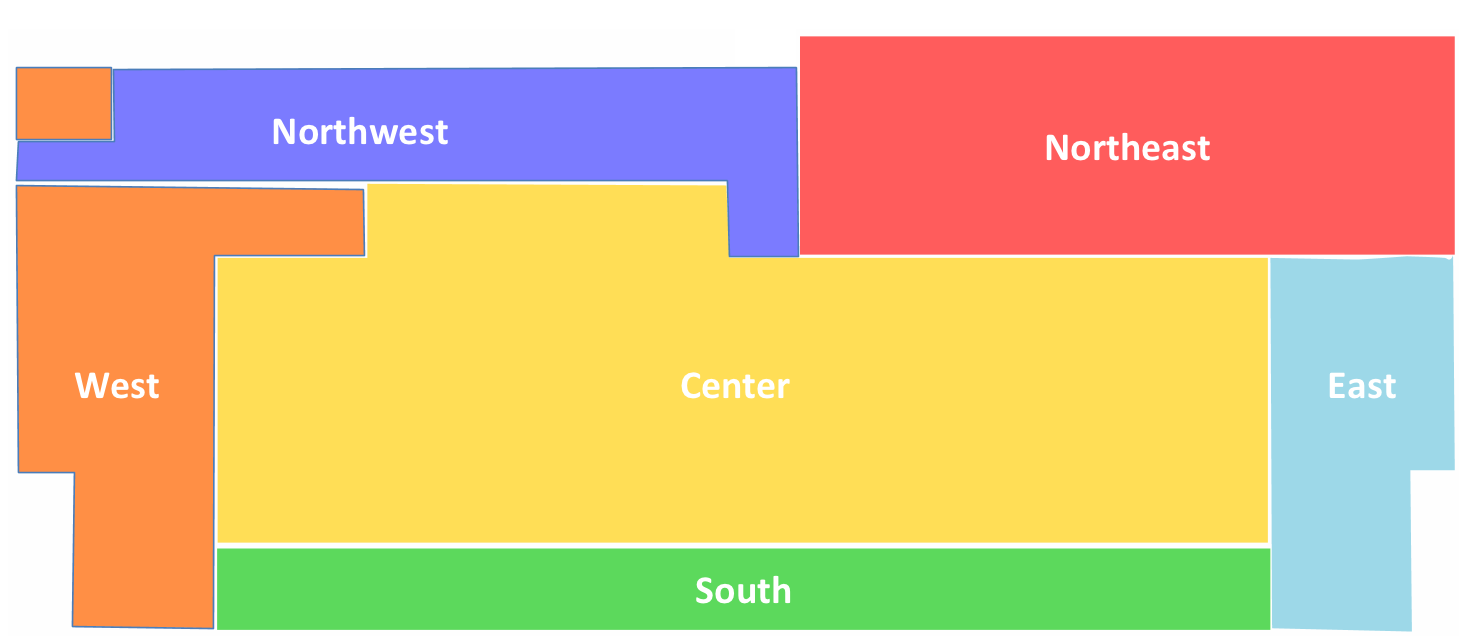
\includegraphics[scale=0.30]{chapters/building_exp/figures/FloorPlan.png}
\vspace*{-0.05cm}
\caption{Zones for the fourth floor of Sutardja Dai Hall.}
\label{fig:floor_plan}
\vspace*{-0.45cm}
\end{figure}


%%%%%%%%%%%%%%%%%%%%%%%%%%%%%%%%%%%%%%%

\subsubsection{Control Scheme}\label{sec:control_scheme}
%\textcolor{red}{schematic of 2 level control.}
SDH is equipped with the Siemens' APOGEE system -- a BAS that controls the building's HVAC system and lighting based on existing control loops. %and allows operators to modify setpoints of various controllers of the HVAC system and monitor its performance via a user interface. 
The communication between the building automation devices is enabled by a building automation and control network (BACnet). 
We develop an external frequency regulation controller to read measurements from and send control commands to the HVAC equipment via the BACnet. 

Our goal is to adjust the instantaneous power consumption of the supply fans to provide frequency regulation while maintaining the indoor temperature on the fourth floor within the comfort zone.
We propose to control the supply fans' power consumption by adjusting their speed and use the airflow rates to the fourth floor for the comfort goal.
The airflow rates to the rooms are chosen not to depend on the frequency regulation signal because they have very different reaction times: the regulation signal is updated every 2 seconds, however the dampers in the VAV boxes have a  time constant in the order of minutes.
Consequently, our controller overrides the BAS' supply fans' speed control loops and the airflow rate control loops at the VAV boxes situated on the fourth floor. 
All other BAS' control loops are left intact.
%In the proposed control architecture, a regulation reference signal,
%denoted by ?Pr, will be transmitted to each participating building.
%We take the ACE (Area Control Error), which indicates
%the imbalance in the grid [9], scale it down by a scaling factor
%and feed it through a bandpass filter to define ?Pr.
Our proposed control architecture consists of a High Level Controller and a Low Level Controller as depicted in Figure \ref{fig:control_scheme}:
%briefly describe below (details can be found in Section \ref{sec:control}).

\begin{itemize}
	\item{High Level Controller (HLC) - Reserve Scheduling and Room Temperature Control}\label{sec:high_level}

A closed-loop Model Predictive Controller (MPC) that operates every hour. Its objective is two-fold: first, determine the reserve capacity that the building can reliably offer for the next operating hour; second, calculate the baseline airflow rate to each room that ensures occupant comfort while providing this amount of reserves.
Both the capacity and the baseline are chosen to minimize electricity cost and maximize rewards from reserve provision.

	\item{Low Level Controller (LLC) - Frequency Tracking}\label{sec:low_level}

A switched controller that modulates the speed of the supply fan every 4 seconds so that its power consumption deviations from its baseline tracks the frequency regulation signal.
It consists of a model-based feedforward controller and a Proportional Integral (PI) feedback controller.
As explained in Section \ref{sec:llc}, our switched controller has a different switching condition from \cite{Vrettos:2016flexlab1}, which makes our controller suitable for scenarios where the building is subject to larger disturbances.  

Note that although PJM's regulation signal is updated every 2 seconds, power consumption measurements of the supply fans in SDH are only available every 10-20 seconds, therefore the LLC was chosen to run at an intermediate rate of 4 seconds. This is a restriction of our particular building. Using another building whose supply fans' power measurements are updated more frequently would only improve our controller's tracking performance.
\end{itemize}


\begin{figure}[t]
\centering
%\vspace*{-0.4cm}
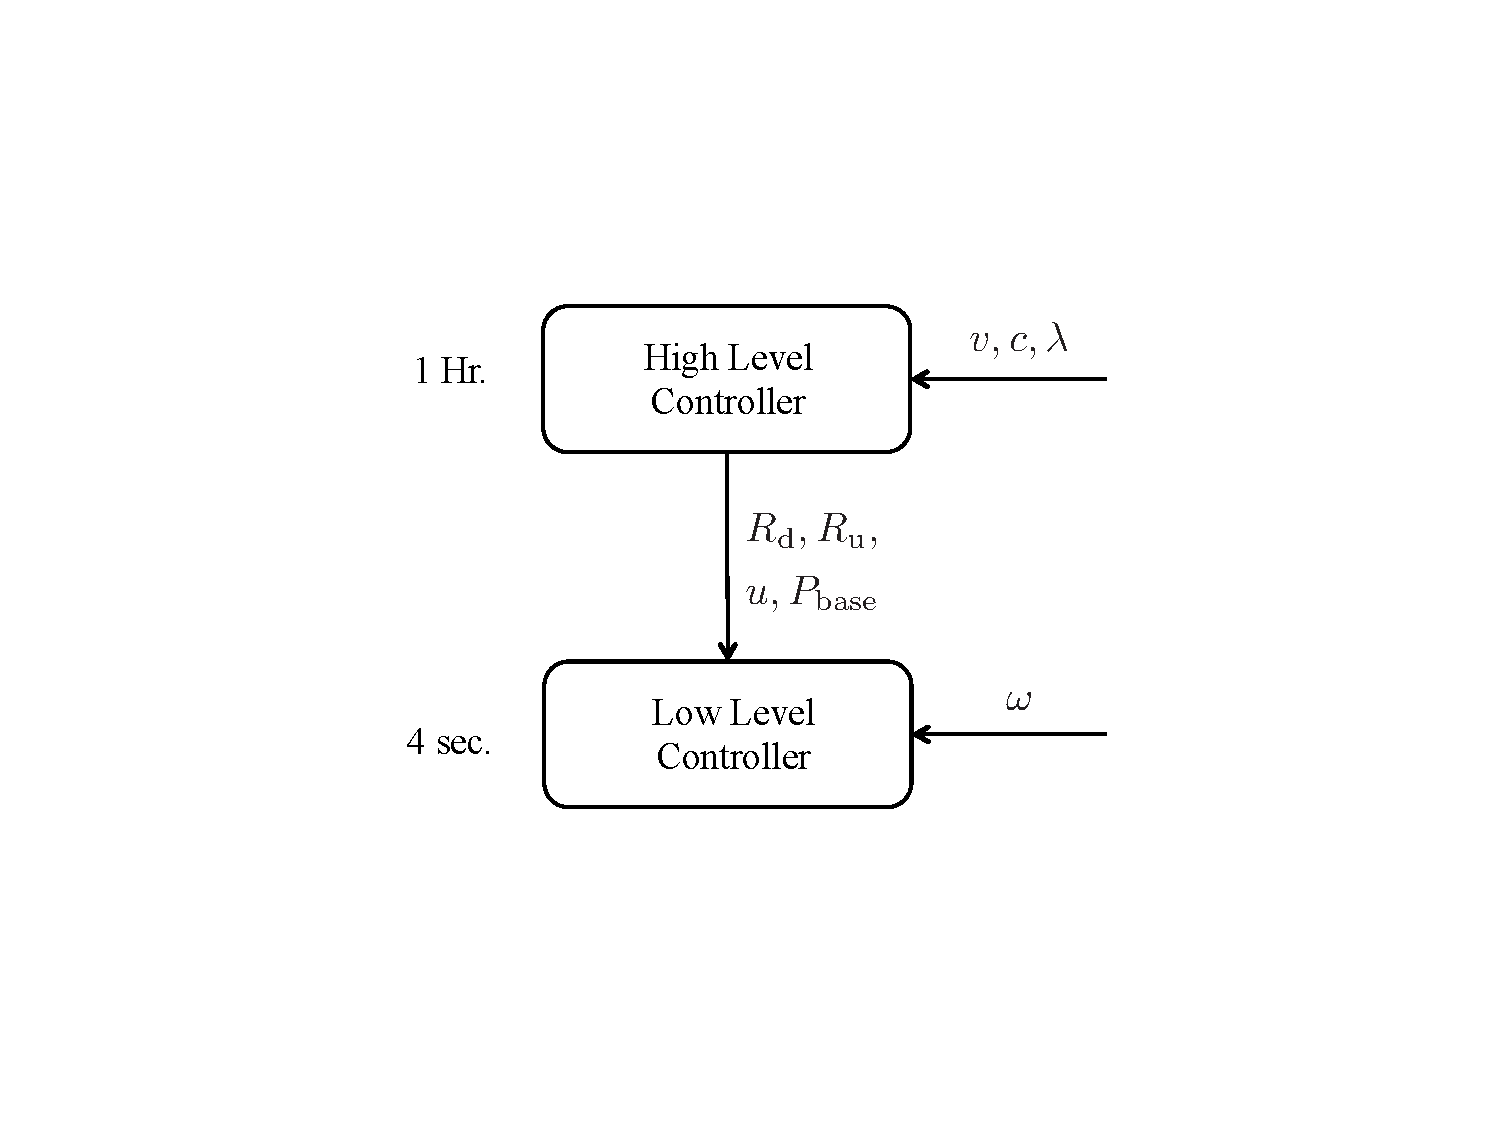
\includegraphics[scale=0.45]{chapters/building_exp/figures/control_scheme.pdf}
\vspace*{-0.05cm}
\caption{Two level control scheme for frequency regulation. See Table \ref{tab:notation} for description of symbols.}
\label{fig:control_scheme}
\vspace*{-0.45cm}
\end{figure}

\begin{table}[b]
\centering
\caption{Table of notation.}
\label{tab:notation}
\begin{tabular}{ll}
\toprule
Symbol & Description \\ \hline
$R_{\text{u}}, R_{\text{d}}$ & Up- and down-regulation capacities \\
$P_{\text{base}}, P$ & Baseline and actual fan power consumption\\
$N_{\text{base}}, N$ & Baseline and actual fan speed\\
$x$ & Zone temperature\\
$u$ & Control input\\
$v$ & Disturbance\\%: ambient air temp., supply air temp.\\
$q$ & Internal gains\\
$w$ & Normalized frequency regulation signal\\
$c$ & Unit electricity cost\\
$\lambda$ & Reward for reserve provision\\
\bottomrule
\end{tabular}
\end{table}


%
%\begin{table}[b]
%\centering
%\begin{tabular}{ll}
%\toprule
%Symbol & Description \\ \hline
%$R_{\text{u},k}, R_{\text{d},k}$ & Up- and down-regulation capacities \\
%$P_{\text{base},k}, P_k$ & Baseline and actual fan power consumption\\
%$N_{\text{base},k}, N_k$ & Baseline and actual fan speed\\
%$x_k$ & Zone temperature\\
%$u_k$ & Control input\\
%$v_k$ & Disturbance\\
%$q_k$ & Internal gains\\
%$w_k$ & Normalized frequency regulation signal\\
%$c_k$ & Unit electricity cost\\
%$\lambda_k$ & Reward for reserve provision\\
%\bottomrule
%\end{tabular}
%\caption{Table of notation.}
%\label{tab:notation}
%\end{table}









%%%%%%%%%%%%%%%%%%%%%%%%%%%%%%%%%%%%%%%%%%%%%%%%%%%%%%%%%%%%%%%
%
% Introduction.tex (part of thesis.tex)
% author: Qie Hu
%
%%%%%%%%%%%%%%%%%%%%%%%%%%%%%%%%%%%%%%%%%%%%%%%%%%%%%%%%%%%%%%%

%!TEX root = ../../thesis.tex

\section{Model Identification}\label{sec:model_id}

\subsection{Building Model}
The data-driven model identified for the fourth floor of SDH in Chapter \ref{chapter:building_model} is used here in our field experiments.
To recap, we model the room temperature evolution as follows:
\begin{equation}
\begin{aligned}\label{eq:building_model}
x_{k+1} &= A x_k + B u_k + C v_k + q_k, \\
\end{aligned}
\end{equation}
where $x \in \mathbb{R}^6$ represents the average temperature in each of the six zones on the fourth floor (see Figure \ref{fig:floor_plan}), $u \in \mathbb{R}^6$ is the input vector that contains the total airflow to each zone, $v:= \left[ v_\text{Ta}, v_\text{Ts} \right]^\top \in \mathbb{R}^2$ is a disturbance vector that describes ambient air temperature and the HVAC system's SAT and  $q \in \mathbb{R}^6$ represents the internal gains due to occupancy and electric devices.
Finally, $A$, $B \in \mathbb{R}^{6\times6}$ and $C \in \mathbb{R}^{6\times2}$ are coefficient matrices.


%%%%%%%%%%%%%%%%%%%%%%%%%%%%%%%%%%%%%%%%%%%%%%
%%%%%%%%%%%%%%%%%%%%%%%%%%%%%%%%%%%%%%%%%%%%%%
%%%%%%%%%%%%%%%%%%%%%%%%%%%%%%%%%%%%%%%%%%%%%%
%%%%%%%%%%%%%%%%%%%%%%%%%%%%%%%%%%%%%%%%%%%%%%


\subsection{Fan Model}

A fan model is identified from 6 weeks of one-minute resolution data for the supply fans collected from sMAP.
The fan laws state that the airflow rate through the fan is proportional to the fan speed, and the fan power is a cubic function of its speed \cite{Hvac_book}. 
Figure \ref{fig:fan_model} confirms the linear relationship between the airflow rate and the fan speed. 
The same figure also shows that there is little difference between the best fit quadratic and cubic curves for the relationship between the fan power and fan speed, suggesting that for the range of fan speeds plotted, a quadratic function can describe this relationship without significant loss of accuracy compared to a cubic function. %for fan speed between 28\% and 90\% of its maximum.
%The best fit quadratic and cubic curves for the relationship between the fan power and fan speed are also shown in the figure and they suggest that a quadratic function is able to describe this relationship without significant loss of accuracy compared to a cubic function. 
Since a quadratic function would simplify the subsequent controller design problem, it is adopted in this work. 
%Assume both supply fans are controlled to the same speed. 
%Let $N$ denote the fan speed of both fans, $u$ the total airflow rate through the fans and $P$ the total power consumption of the fans, then the fan model is defined as follows:
Let $N$ denote the fans' speed, $u$ the total airflow through the fans and $P$ the total fan power consumption, then the fan model is given as follows:
\begin{equation}\label{eq:fan_model}
\begin{aligned}
N & = f(u) = a_1 u + a_2\\
P & = g(N) = b_1 N^2 + b_2 N + b_3\\
P & = h(u) = c_1 u^2 + c_2 u + c_3.\\
\end{aligned}
\end{equation} 

\begin{figure}[h]
\centering
\vspace*{1cm}
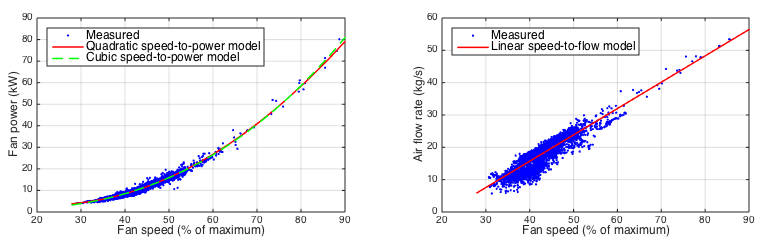
\includegraphics[width=\textwidth]{chapters/building_exp/figures/fan_model.png}
\caption{Fan measurements and identified models for fan power and air flow as functions of fan speed.}
\label{fig:fan_model}
\vspace*{-0.15cm}
\end{figure}









%%%%%%%%%%%%%%%%%%%%%%%%%%%%%%%%%%%%%%%%%%%%%%%%%%%%%%%%%%%%%%%
%
% Introduction.tex (part of thesis.tex)
% author: Qie Hu
%
%%%%%%%%%%%%%%%%%%%%%%%%%%%%%%%%%%%%%%%%%%%%%%%%%%%%%%%%%%%%%%%

%!TEX root = ../../thesis.tex

\section{Two-Level Control Scheme}\label{sec:control}


\subsection{High Level Controller}\label{sec:hlc}
\subsubsection{Regulation Capacities}

Let $P_{\text{base}}$ and $u_{\text{base}}$ represent the power consumption of the supply fans and the airflow rate through the fans at the baseline operating point. Then,
\begin{equation}\label{eq:P}
\begin{aligned}
P_{\text{base}}(k) &= h\big(u_{\text{base}}(k)\big)\\
&=h\big(1^\top u(k) + v_{\dot{\text{m}}}(k)\big),
\end{aligned}
\end{equation}
where $u(k) \in \mathbb{R}^6$ represents the controlled airflow rates to the six zones on the fourth floor, and $v_{\dot{\text{m}}}(k) \in \mathbb{R}$ is a disturbance that represents the total airflow rate to the remaining floors.
Now, define $R_{\text{u}}(k)$ and $R_{\text{d}}(k)$ as the up- and down-regulation capacities at time step $k$, respectively\footnote{For demand resources, up-regulation requires a reduction in its power consumption and down-regulation requires an increase in consumption.}. In addition, let $r_{\text{u}}(k)$ and $r_{\text{d}}(k)$ denote the maximum changes in fan speed at time step $k$ as a result of reserve provision. Then, the regulation capacities are as follows

\begin{equation}\label{eq:Ru_Rd}
\begin{aligned}
R_{\text{u}}(k) & = P_{\text{base}}(k) - P_{\text{u}}(k)\\
 & = h\big(u_{\text{base}}(k)\big) - g\big(f(u_{\text{base}}(k)) - r_{\text{u}}(k)\big)\\
R_{\text{d}}(k) & = P_{\text{d}}(k) - P_{\text{base}}(k)\\
 & = g\big(f(u_{\text{base}}(k)\big) + r_{\text{d}}(k)) - h\big(u_{\text{base}}(k)\big),
\end{aligned}
\end{equation}
\noindent
where $P_{\text{u}}$ and $P_{\text{d}}$ denote the fans' power consumption when providing maximum up- and down-regulation capacities, respectively.

During real-time operation, the building receives a normalized real-time regulation signal $\omega \in [-1,1]$ from PJM, which represents the requested regulation amount $R$ as a fraction of the declared capacities $R_{\text{u}}$ and $R_{\text{d}}$. In other words, the building must control its power consumption $P$ at time $k$ to track the following reference (desired) value:

\begin{equation}\label{eq:P_ref}
\begin{aligned}
P_{\text{ref}}(k) &= P_{\text{base}}(k)+R(k) \\
	&= P_{\text{base}}(k)+\begin{cases}
	\omega(k) R_{\text{u}}(k) & \mbox{if } \omega(k) < 0 \mbox{ (up-regulation)} \\ 
	\omega(k) R_{\text{d}}(k) & \mbox{if } \omega(k) \geq 0 \mbox{ (down-regulation).} 
	\end{cases} 
\end{aligned}
\end{equation}

%\noindent Finally, PJM requires that each resource's baseline consumption and regulation capacities be declared at the start of every hour and remain fixed for that hour.

%%%%%%%%%%%%%%%%%%%%%%%%%%%%%%%%%%%%%%%%%%%%%%%%%

\subsubsection{Input Constraints}


The airflow rates to the fourth floor must remain fixed for each hour in order to maintain a constant baseline, in addition to being restricted by the minimum and maximum airflow settings of the HVAC system.
Note that in our experiment setup, $u$ is unaffected by the uncertain regulation signal $w$.
%\begin{equation}
\begin{multline}\label{eq:u_constraint_const}
u(k) = u(k+j) \text{~~for all~} k = 4m+1,~ j = \{1,2,3\}, m \leq n/4-1, ~m \in \mathbb{N},
\end{multline}
%\end{equation} 
\begin{equation}\label{eq:u_constraint}
u_{\text{min}} \leq u(k) \leq u_{\text{max}}.
\end{equation}

Furthermore, there are minimum and maximum fan speed requirements: $N_\text{min} = 20\%$ and $N_\text{max} = 60\%$, where the maximum limit ensures that the HVAC system's duct static pressure remains under the maximum safe value of 2 inches water column, and the minimum limit ensures that the supply fans have sufficient power to drive the supply air throughout the building: 
\begin{equation}\label{eq:N_constraint}
N_\text{min} \leq N(k) \leq N_\text{max} \text{~for all~} \omega(k) \in [-1,1],
\end{equation}
where $N(k)$ is the fan speed at time step $k$.
Since $\omega$ is unknown at scheduling time, the above constraint must hold for any $\omega$. 
The fan model states that $N$ is given by the inverse of the speed-to-power function, $N = g^{-1}(P)$, which is usually complex, however, it has a simple form at the boundary values of $\omega$:
\begin{equation}\label{eq:N_w}
N(k) = \begin{cases}
	N_{\text{base}}(k) - r_{\text{u}}(k) & \mbox{if } \omega(k) = -1 \\ 
	N_{\text{base}}(k) + r_{\text{d}}(k) & \mbox{if } \omega(k) = 1. \\ 
	\end{cases} 
\end{equation}
Thus, the above constraints can be satisfied by imposing the following robustified version of \eqref{eq:N_constraint}
\begin{equation}\label{eq:N_constraint_rob}
N_\text{min} + r_u \leq N_{\text{base}}(k) \leq N_\text{max} - r_d.
\end{equation}
Although \cite{Vrettos:2016flexlab1} showed that the energy content of $\omega$ over a 15 minute interval is typically limited and $\omega \in [ -\omega_{\text{lim}}, \omega_{\text{lim}}]$ most of the time, where $0<\omega_{\text{lim}} < 1$;
we choose to deal with the uncertainty introduced by $\omega$ in a robust fashion, by accounting for the worst case, i.e., $\omega = \pm 1$.
This way, the building need not make any assumptions on the statistical properties of $\omega$, and it has the added advantage of building additional robustness to modeling and forecast uncertainties for an occupied building.

%%%%%%%%%%%%%%%%%%%%%%%%%%%%%%%%%%%%%%%%%%%%%%%%%

\subsubsection{Output Constraints}

The indoor temperature $x$ should be kept within the time varying comfort zone $[x_{\text{min}}(k), x_{\text{max}}(k)]$ for all $k$:
\begin{equation}
x_{\text{min}}(k) \leq x(k) \leq x_{\text{max}}(k).
\end{equation}
Note that $x$ is unaffected by the unknown signal $\omega$ since $u$ is independent of $\omega$.


%Since we choose $u(k)$ independently from the unknown signal $\omega(k)$ and the zone temperatures $x(k)$ are given by \eqref{eq:building_model}, then $x(k)$ is also unaffected by $w(k)$. 
%Therefore to maintain the indoor temperatures within the time varying comfort zone $[x_{\text{min}}(k), x_{\text{max}}(k)]$, we simply impose
%\begin{equation}
%x_{\text{min}}(k) \leq x(k) \leq x_{\text{max}}(k).
%\end{equation}

The regulation capacities are required to be fixed for each hour which translates to the following constraint:
\begin{multline}\label{eq:R_constraint_const}
R_{\text{u}}(k) = R_{\text{u}}(k+j) \text{~and~} R_{\text{d}}(k) = R_{\text{d}}(k+j)\\
\text{~for all~} k = 4m+1,~ j = \{1,2,3\}, m \leq n/4-1, ~m \in \mathbb{N}.
\end{multline}

\noindent In addition, these capacities must be non-negative.
Because fan power is a non-decreasing function of its speed in the operating range $[N_\text{min}, N_\text{max}]$, the following condition ensures $R_{\text{u}}(k) \geq 0$ and $R_{\text{d}}(k) \geq 0$:
\begin{equation}\label{eq:r_constraint} 
r_{\text{u}}(k) \geq 0, ~r_{\text{d}}(k) \geq 0.
\end{equation}

%Furthermore, the regulation capacities must be fixed for each hour and be non-negative, i.e., $R_{\text{u}}(k) \geq 0$ and $R_{\text{d}}(k) \geq 0$. 
%Similar to the constant baseline restriction for each hour, the first requirement can be met by applying the following constraint
%\begin{multline}\label{eq:R_constraint_const}
%R_{\text{u}}(k) = R_{\text{u},k+j} \text{~and~} R_{\text{d}}(k) = R_{\text{d},k+j}\\
%\text{~for all~} k = 4m+1,~ j = \{1,2,3\}, \\
%m \leq n/4-1, ~m \in \mathbb{N}.
%\end{multline}
%To meet the second requirement, we constrain the deviations in the fan speed as a result of reserve provision as follows
%\begin{equation}\label{eq:r_constraint} 
%r_{\text{u}}(k) \geq 0, ~r_{\text{d}}(k) \geq 0.
%\end{equation}
%Since fan power is a non-decreasing function of its speed in the operating range $[N_\text{min}, N_\text{max}]$, the above constraint results in $R_{\text{u}}(k) \geq 0$ and $R_{\text{d}}(k) \geq 0$. 

%%%%%%%%%%%%%%%%%%%%%%%%%%%%%%%%%%%%%%%%%%%%%%%%%

\subsubsection{Cost Function}
The objective of the HLC is to choose the HVAC's operating point to minimize the cost of electricity consumption and maximize rewards from reserve provision. 
%Conceptually, a building should have a higher baseline consumption so that it has more room to reduce its power consumption to provide more up-regulation capacity. Similarly, to provide more down-regulation requires a lower baseline. However, a high baseline consumption also translates to higher electricity cost. Therefore, there is a trade-off.
\begin{assumption}
Electricity cost is calculated based on the baseline consumption.
\end{assumption}
\begin{assumption}
The payment for both up- and down-regulations are the same.
\end{assumption}
Then, the building's objective is to minimize the following cost function
\begin{equation}\label{eq:cost_function}
c(k) P_{\text{base}}(k) - \lambda(k) \big(R_{\text{u}}(k) + R_{\text{d}}(k)\big),
\end{equation}
where $c$ denotes the unit electricity cost and $\lambda$ denotes the reward for providing regulation service.

%%%%%%%%%%%%%%%%%%%%%%%%%%%%%%%%%%%%%%%%%%%%%%%%%

\subsubsection{Robust Optimization Problem}

We introduce the following robust optimization problem:
\begin{equation}\label{eq:opt}
\begin{aligned}
& \underset{u(k), r_{\text{u}}(k), r_{\text{d}}(k)}{\text{minimize}} 
%& & \textstyle\sum_{k=1}^{n} c(k) h(1^\top u(k) + v_{\dot{\text{m}}}(k)) - \lambda(k) (R_{\text{u}}(k) + R_{\text{d}}(k)) \nonumber\\
& & \textstyle\sum_{k=1}^{n} c(k) P_{\text{base}}(k) - \lambda(k) \big(R_{\text{u}}(k) + R_{\text{d}}(k)\big) \\
& \text{subject to}
& & u_{\text{min}} \leq u(k) \leq u_{\text{max}} \\%, \forall k \\
&&& N_{\text{min}} + r_u \leq N_{\text{base}}(k) \leq N_{\text{max}} - r_d \\
&&& x(k) = Ax(k) + Bu(k) + Cv(k) + q(k) \\
&&& x_{\text{min}}(k) \leq x(k) \leq x_{\text{max}}(k)  \\
%& u_{\text{min},i} \leq u_{i}(k) \leq u_{\text{max},i} ~\text{for}~ i \in \mathcal{I}\\
&&& r_{\text{u}}(k) \geq 0, ~r_{\text{d}}(k) \geq 0\\
%&&&u(k) = u_{k+j} \text{~for all~} k = 4m+1,~ j = \{1,2,3\}, \\
%&&& \quad \quad \text{for all}~ k \\
&&& \text{conditions~} (\ref{eq:u_constraint_const}) \text{~and~} (\ref{eq:R_constraint_const}) \text{~for constant }\\
&&& \quad\quad \text{hourly baseline and regulation capacities}.
\end{aligned}
\end{equation}

\noindent (\ref{eq:opt}) is a deterministic nonlinear optimization, with non-convex quadratic cost function and linear equality and inequality constraints. Despite its non-convexity, it can be solved in Matlab using YALMIP \cite{Lofberg:2004yalmip} and the \textit{fmincon} solver in less than one second, due to its small size. The outcome is the baseline operating point for the HVAC system, and the up- and down-regulation capacities $R_{\text{u}}(k)$ and $R_{\text{d}}(k)$ for each time step in the scheduling horizon $k = 1, \ldots, n$.

%%%%%%%%%%%%%%%%%%%%%%%%%%%%%%%%%%%%%%%%%%%%%%%%%

\subsubsection{Disturbance Approximation and Forecast}
The building's dynamics are subject to the following disturbances: ambient temperature $v_{\text{Ta}}$, SAT $v_{\text{Ts}}$ and internal gains due to occupancy $q$. 
Ambient temperature forecasts are obtained from the publicly available database of \textit{darksky.net} \cite{darksky}. 
Analysis of historical data indicates that SAT rarely varies, as a result, it is measured at each time step $k$ and assumed constant for the HLC horizon, i.e., 1 hour for the certification experiment and 4 hours for the tracking experiment.
The internal gains $q$ is first estimated at each time step $k$ from the building model and real-time measurements, and then assumed constant for the HLC horizon.
In addition, the cost function \eqref{eq:cost_function} is affected by $v_{\dot{\text{m}}}$, the total airflow rate to other floors of SDH, through \eqref{eq:P} and \eqref{eq:Ru_Rd}. This is also measured at each time step $k$ and assumed constant for the HLC horizon.




%%%%%%%%%%%%%%%%%%%%%%%%%%%%%%%%%%%%%%%%%%%%%%%%%
%%%%%%%%%%%%%%%%%%%%%%%%%%%%%%%%%%%%%%%%%%%%%%%%%
%%%%%%%%%%%%%%%%%%%%%%%%%%%%%%%%%%%%%%%%%%%%%%%%%


\subsection{Low Level Controller}\label{sec:llc}

The Low Level Controller (LLC)'s responsibility is to vary the fan power $P$ to track the reference $P_{\text{ref}}$. 
Our approach is different from \cite{Macdonald:2014pjm} which used the frequency of the variable frequency drive as the control input, and from \cite{Lin:2015exp} where control inputs, acting as disturbances, are superimposed onto HVAC's existing control loop commands.

We improve on the switched controller proposed in \cite{Vrettos:2016flexlab1}, so that it is suitable for buildings subjected to large disturbances where an accurate fan model is not available. 
It consists of two sub-controllers. 
Controller 1 is a model-based feedforward controller which uses the fan model from \eqref{eq:fan_model} to determine the fan speed required for a given $P_{\text{ref}}(k)$, i.e., $N(k) = g^{-1}(P_{\text{ref}}(k))$. 
This feedforward controller has a fast response and thus, is best suited when there is a large change in the reference regulation signal, i.e., $|P_{\text{ref}}(k) - P_{\text{ref}}(k-1)|>\epsilon$ where $\epsilon$ is a user defined threshold value. 
On the other hand, Controller 1 has non zero steady state error due to inaccuracies in the fan model. 
Therefore, Controller 2 -- a PI controller, is used to reduce any steady state error from Controller 1. 
%In designing PI controllers, there is a trade-off between small overshoot and fast response rate. 
The implementation of the LLC is presented in Algorithm \ref{alg:llc}.
%Consider a small step change in the reference regulation signal, i.e., i.e., $|\Delta P_{\text{ref}}(k) - \Delta P_{\text{ref},k-1}| \leq \epsilon$, Controller 2 is active and is sufficient to provide good tracking.
%On the other hand,  if the step change in the reference signal is large and $|\Delta P_{\text{ref}}(k) - \Delta P_{\text{ref},k-1}|>\epsilon$, then Controller 1 is activated to quickly bring the fans' power consumption close to the required value.
Step 13 is the discrete implementation of the PI controller, where $\Delta t$ is the discretization time step (4 seconds in our case).
In step 15, the fan speed is capped between $N_\text{min}$ and $N_\text{max}$ to satisfy constraint (\ref{eq:N_constraint}).

\begin{algorithm}
\caption{Low Level Controller}
\label{alg:llc}
\begin{algorithmic}[1]
\State Initialize previous tracking error $e(k-1) = 0$, reference regulation signal $P_{\text{ref}}(k-1)=0$ and fan speed $N(k-1)$ 
\While{experiment is running}
	\State Compute baseline fan power $P_{\text{base}}(k) = h(u_{\text{base}}(k))$
	\State Compute reference (desired) fan power $P_{\text{ref}}(k) = P_{\text{base}}(k)+\omega(k) R_{\text{u}}(k)$ if $\omega(k)<0$ and $P_{\text{ref}}(k) = P_{\text{base}}(k)+\omega(k) R_{\text{d}}(k)$ if $\omega(k) \geq0$
	\State Measure actual fan power $P(k)$
	\State Compute current tracking error $e(k) = P_{\text{ref}}(k) - P(k)$ 
	\If {$|P_{\text{ref}}(k) - P_{\text{ref}}(k-1)|>\epsilon$}
		\State Use model-based controller:
    		\State $N(k) = g^{-1}(P_{\text{ref}}(k))$
    	\Else
		\State Use PI controller:
        	\State $N(k) = N(k-1) + K_\text{P} (e(k)-e(k-1))+\frac{K_\text{P}}{K_\text{I}} e(k) \cdot \Delta t$	
    	\EndIf
	\State Cap fan speed: $N(k) = \max\big(\min(N(k),N_\text{max}),N_\text{min}\big)$
	\State Update variables: $e(k-1) \gets e(k)$, $P_{\text{ref}}(k-1) \gets P_{\text{ref}}(k)$ and $N(k-1) \gets N(k)$
\EndWhile
\end{algorithmic}
\end{algorithm}

The improved performance of our switched controller compared to that in \cite{Vrettos:2016flexlab1} is a result of the new switching condition. 
In \cite{Vrettos:2016flexlab1}, the LLC switches between its sub-controllers based on whether the absolute tracking error is greater than a threshold $\bar{\epsilon}$, i.e., $|e(k)|>\bar{\epsilon}$. 
To see why this controller may fail when an accurate fan model is not available, consider a step change in the reference signal $P_{\text{ref}}$ at time step $k$ such that $|e(k)|>\bar{\epsilon}$. 
According to the switching condition in \cite{Vrettos:2016flexlab1}, Controller 1 would become active.
If the fan model is accurate enough such that the fan speed given by the inverse fan model is able to reduce the tracking error at the next time step $k+1$ to $|e(k+1)| \leq \bar{\epsilon}$, then Controller 2 would take over and continue to decrease the tracking error from time $k+1$ onwards.
On the other hand, if the fan model is not accurate enough such that $|e(k+1)| > \bar{\epsilon}$, then the switched controller in \cite{Vrettos:2016flexlab1} is stuck in Controller 1 with a constant fan speed $N(k) = g^{-1}(P_{\text{ref}}(k))$, %unless $P_{\text{base}}(k)$ or $\Delta P_{\text{ref}}(k)$ changes. 
and consequently, a constant tracking error whose absolute value is greater than $\bar{\epsilon}$.
In practice, accurate fan models are often not available for commercial buildings like SDH which are subject to large disturbances and uncertainties. 
Therefore, larger values of $\bar{\epsilon}$ are needed to avoid the above problem. 
We found that for SDH, the required value of $\bar{\epsilon}$ would be so large that the switched controller essentially acts as a simple PI controller, and a PI controller alone is unable to achieve the fast response necessary for a good tracking performance.%frequency regulation signal tracking.

Our proposed switched controller overcomes the above problem and is therefore suitable for buildings where an accurate fan model is not available. Consider the above scenario again, $|P_{\text{ref}}(k+1) - P_{\text{ref}}(k)| = 0 \leq \epsilon$ independent of the fan model, therefore Controller 2 is activated at time step $k+1$ and continues to reduce the tracking error.




%%%%%%%%%%%%%%%%%%%%%%%%%%%%%%%%%%%%%%%%%%%%%%

\subsubsection{PI Controller Tuning}\label{sec:PItuning}
The proportional $K_\text{P}$ and integral gains $K_\text{I}$ of the PI controller are calculated using the %Chien, Hrones and Reswick
Open Loop Ziegler Nichols method \cite{Moderncontrol_book}. Open loop responses of the fan power to step changes in its speed were recorded. 
The delay time and time constant of the response were used to compute the gains $K_\text{P}$ and $K_\text{I}$.
These values served as initial guesses, which we fine tuned later through trial and error. 
The final gain values are: $K_\text{P} = 0.3$, $K_\text{I} = 6.8$.

Note that the Closed Loop Ziegler Nichols tuning method used in \cite{Vrettos:2016flexlab1} may be unsafe for a regular building, because it requires increasing the proportional gain $K_\text{P}$ until the fan power exhibits sustained oscillations, i.e., the system is marginally stable.
Also note that a single PI controller for the entire operating range of the supply fans was found to be sufficient to achieve good tracking performance.
















%%%%%%%%%%%%%%%%%%%%%%%%%%%%%%%%%%%%%%%%%%%%%%%%%%%%%%%%%%%%%%%
%
% Introduction.tex (part of thesis.tex)
% author: Qie Hu
%
%%%%%%%%%%%%%%%%%%%%%%%%%%%%%%%%%%%%%%%%%%%%%%%%%%%%%%%%%%%%%%%

%!TEX root = ../../thesis.tex

\section{Experimental Results}\label{sec:results}


%%%%%%%%%%%%%%%%%%%%%%%%%%%%%%%%%%%%%%%%%%%%%%%%%%%
%%%%%%%%%%%%%%%%%%%%%%%%%%%%%%%%%%%%%%%%%%%%%%%%%%%

\subsection{Communication Architecture}\label{sec:comm}

The communication architecture is shown in Figure \ref{fig:comm_architecture}.
The HLC is implemented in Matlab on a standard laptop and the LLC is implemented in Python on a server located in SDH.
The Matlab and Python scripts communicate asynchronously via local port forwarding and TCP/IP.
All requests are initiated from the Matlab script and forwarded to the connected port on the laptop, while the Python script continuously listens to the corresponding port on the server and responds to any received requests.

The HLC queries the publicly available database of forecast.io to obtain weather forecasts, and collects building measurements by sending read requests to the Python script, which directly queries the BACnet to obtain these measurements. 
At the same time, the HLC computes the regulation capacities, baseline and optimal airflow rate setpoints and sends them as write requests to the Python script. The script then updates the values of its local copy of the regulation capacities and baseline, and adjust actuator setpoints via BACnet.
Finally, the LLC reads preloaded PJM regulation signal, then determines and adjusts the fan speed setpoint using read and write requests via the BACnet.  

\begin{figure}[t]
\centering
%\vspace*{-0.4cm}
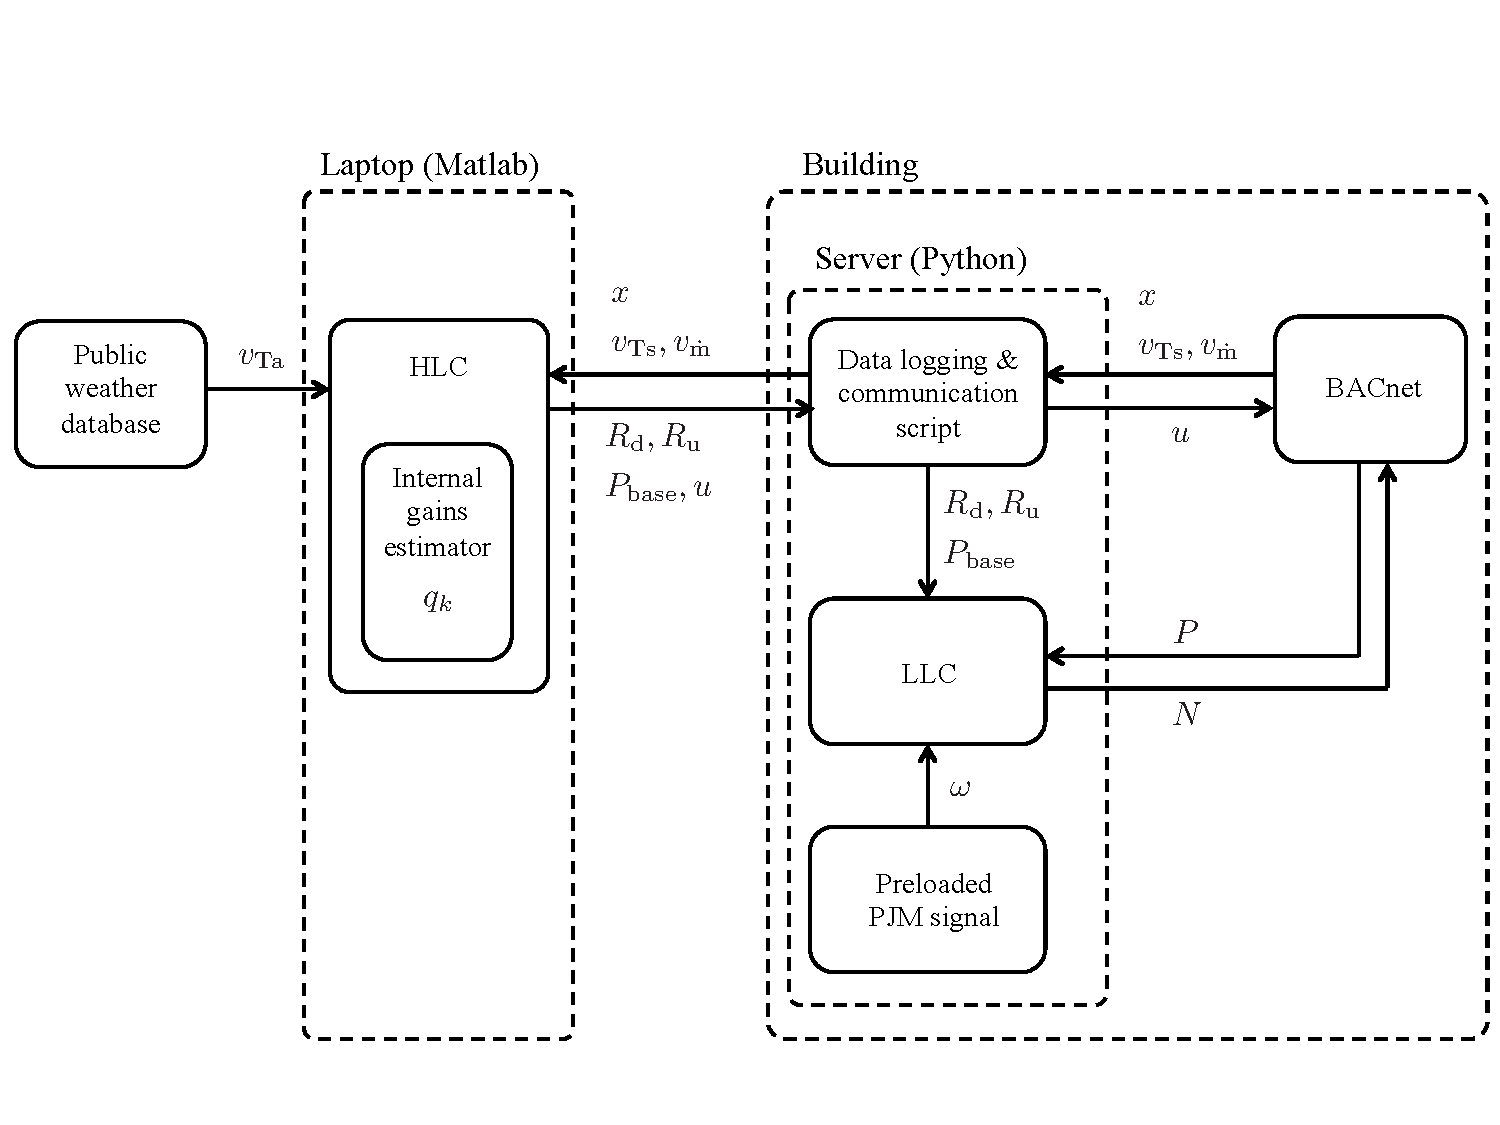
\includegraphics[width = \textwidth]{chapters/building_exp/figures/comm_architecture.pdf}
%\vspace*{-0.5cm}
\caption{Communication architecture. See Table \ref{tab:notation} for description of symbols.}
\label{fig:comm_architecture}
\vspace*{-0.45cm}
\end{figure}


%%%%%%%%%%%%%%%%%%%%%%%%%%%%%%%%%%%%%%%%%%%%%%%%%%%
%%%%%%%%%%%%%%%%%%%%%%%%%%%%%%%%%%%%%%%%%%%%%%%%%%%


\subsection{Performance Metric}\label{sec:performance_metric}

PJM's composite performance score $S_\text{comp}$ is used to evaluate our controller's performance in following the regulation signal. 
This score consists of three equally weighted components: a correlation score $S_\text{c}$, a delay score $S_\text{d}$ and a precision score $S_\text{p}$, defined as in \cite{PJM12}:

\begin{equation}\label{eq:pjm_score}
\begin{aligned}
S_\text{c} = & \max_{t \in [0, 5 \text{min}]} (\sigma_t) \\
S_\text{d} = & \frac{1}{5 \text{min}} \left(5 \text{min} - \frac{\max(t^\star - 10 \text{sec},0)}{60\text{sec}}\right) \\
& \text{where}~t^\star =  \arg\max_{t \in [0, 5 \text{min}]} (\sigma_t)\\
S_\text{p} = & 1 - \frac{1}{n_h} \sum_{k=1}^{n_h}  \frac{\left | P_{\text{ref},k} - P_{k}\right |}{0.5\cdot(R_{\text{d},h} + R_{\text{u},h})}  \\
S_\text{comp} = & \frac{1}{3} \cdot \left( S_\text{c} + S_\text{d} + S_\text{p} \right).\\
\end{aligned}
\end{equation}

In \eqref{eq:pjm_score}, $\sigma_t$ represents the correlation between the reference signal $P_{\text{ref},k}$ and the fans' actual power consumption delayed by $t$ seconds $P_{k+t}$. In other words, $S_\text{c}$ measures the maximum correlation between the regulation signal and the building's response signal within each 5 minute window. $S_\text{d}$ represents the response delay when maximum correlation occurs with a ``free'' 10 second allowance, and $S_\text{p}$ measures the average tracking error scaled by the building's regulation capacity offered for that hour $h$.
All scores take values between 0 and 1, with 1 being a perfect score. 
Following PJM's rules, we generate $S_\text{c}$ and $S_\text{d}$ every 10 seconds and calculate $S_\text{p}$ once per hour.
The performance score $S_\text{comp}$ is then computed every hour by averaging $S_\text{c}$ and $S_\text{d}$ scores for the hour and using $S_\text{p}$ for that hour.



%%%%%%%%%%%%%%%%%%%%%%%%%%%%%%%%%%%%%%%%%%%%%%%%%%%
%%%%%%%%%%%%%%%%%%%%%%%%%%%%%%%%%%%%%%%%%%%%%%%%%%%

\subsection{Certification Experiment}\label{sec:certification_exp}
Any resource that intends to participate in PJM's regulation market must first pass the certification test, which is run during a continuous 40-minute period, using the test signal published on PJM's website \cite{PJM_signal_price}.
The test is scored using $S_\text{comp}$ evaluated on the entire 40-minute test period, and a resource is certified only after it achieves three consecutive scores of 0.75 or above.
Finally, both the baseline consumption and regulation capacity must be declared before the test begins and remain constant throughout the test.

%The resource must set and hold for the test duration the MW-value base point that the resource is regulating around. Changes in base loading for a resource during the test period invalidates the test. Once the test is announced, a resource is not permitted to change its regulation capacity.

%The first of these test may be performed internally by the member following the PJM Regulation test procedure. The remaining tests should be administered by PJM Dispatch.

We carried out four certification tests at various hours of the day from November 27 (Sunday) to 28 (Monday), 2016 and achieved $S_\text{comp}$ values around 0.9 in all tests (Table \ref{tab:certification}). This demonstrates that our controller's performance is robust to disturbances such as weather and occupancy. 
Figure \ref{fig:cert_power} shows the desired reference signal $P_{\text{ref}}$, the fan's actual power consumption $P$ and the percentage tracking error defined as $(P_\text{ref} - P)/P_\text{ref} \cdot 100 $ for the test conducted on November 28 starting at 10~a.m.. An absolute tracking error of less than 28\% is observed during 90\% of the test period.

\begin{table}[b]
\centering
\begin{tabular}{c | c | c c c | c}
\toprule
Test date & Test start time & $S_\text{c}$ & $S_\text{d}$ & $S_\text{p}$ & $S_\text{comp}$  \\ \hline
Nov 27 & 22 hours & 0.90 & 0.90 & 0.88 & 0.89\\
Nov 28 & 10 hours & 0.93 & 0.93 & 0.88 & 0.91 \\
Nov 28 & 13 hours & 0.92 & 0.90 & 0.89 & 0.90 \\
Nov 28 & 16 hours & 0.93 & 0.92 & 0.89 & 0.91 \\
\bottomrule
\end{tabular}
\caption{PJM performance scores for certification tests.}
\label{tab:certification}
\end{table}

\begin{figure}[t]
\centering
%\vspace*{-0.4cm}
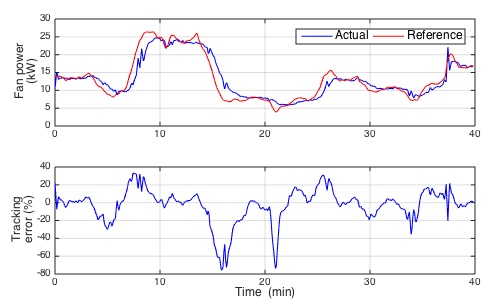
\includegraphics[scale=0.7]{chapters/building_exp/figures/Cert_power.png}
%\vspace*{-0.5cm}
\caption{Certification experiment results: power and tracking error.}
\label{fig:cert_power}
%\vspace*{-0.45cm}
\end{figure}


%%%%%%%%%%%%%%%%%%%%%%%%%%%%%%%%%%%%%%%%%%%%%%%%%%%
%%%%%%%%%%%%%%%%%%%%%%%%%%%%%%%%%%%%%%%%%%%%%%%%%%%

\subsection{Tracking Experiment}\label{sec:tracking_exp}
In this section, we present the results from the tracking experiment conducted from 13:00 to 17:00 on Nov 29, 2016, which uses the historic PJM RegD signal recorded from 13:00 to 17:00 on July 1, 2016 \cite{PJM_signal_price} as the reference frequency regulation signal.

After successful certification, each resource must maintain a historic performance score $S_\text{comp}$ of above 40\% to continue to provide regulation services. In addition, a resource must achieve an average hourly score of at least 50\% to receive payments for offering regulation capacity. 
Table \ref{tab:tracking} shows the $S_\text{comp}$ scores calculated for each hour, as well as the average scores, of our tracking experiment.
Our controller scored $S_\text{comp}$ values well above both thresholds during the field experiment, demonstrating good tracking performance. 

%Regulating resources that have not met performance thresholds over a specified time period will be disqualified and must re-qualify to offer into the regulating market. The disqualification threshold is based on the historic performance score. The historic performance score is a rolling average actual hourly performance score for the last 100 hours a resource has operated. When the historic performance score falls below 40\%, the resource will no longer be eligible to offer into the regulation market.

\begin{table}[b]
\centering
\begin{tabular}{c | c c c | c}
\toprule
 & $S_\text{c}$ & $S_\text{d}$ & $S_\text{p}$ & $S_\text{comp}$  \\ \hline
1\textsuperscript{st} hour & 0.94 & 0.91 & 0.99 & 0.95\\
2\textsuperscript{nd} hour & 0.72 & 0.52 & 0.99 & 0.74 \\
3\textsuperscript{rd} hour & 0.63 & 0.63 & 0.99 & 0.75 \\
4\textsuperscript{th} hour & 0.62 & 0.31 & 0.99 & 0.64 \\ %\hline
Mean & 0.73 & 0.59 & 0.99 & 0.77 \\
\bottomrule
\end{tabular}
\caption{PJM performance scores for tracking experiment.}
\label{tab:tracking}
\end{table}

Figure \ref{fig:track_power} shows that the actual fan power is regulated to closely track the reference power signal. Indeed, an absolute tracking error of less than 16\% is achieved 90\% of the time. The error is greatest at the start of the experiment as the fans switch from normal operation to frequency regulation mode, and decays as the experiment progresses.
The fans offer a constant total regulation capacity of 23.3 kW every hour, % This is because the constraints on fan speed (N_min and N_max) are active at the optimal solution, which translates to fixed power difference P(N_max) - P(N_min).
but the split between up- and down-regulation capacities varies hourly as the building's baseline consumption changes. 
Finally, we confirm that the duct static pressure remains below the maximum limit of 2 inches water column throughout the experiment.

We present the zone temperatures and airflow rates from the experiment in Figure \ref{fig:track_temp_flow}, and note the following observations. 
First, all zone temperatures are maintained within the comfort bounds and flow rates are kept within the permissible ranges. 
Second, to minimize electricity cost, flow rates are kept at their minima unless continued supply of minimum airflow rate to a zone is predicted to cause the zone temperature to exceed its maximum limit within the prediction horizon. 
For example, flow rates are increased in the second and third hours for the West zone to maintain occupant comfort. 
Third, observe that temperatures decrease during the third hour in the West zone and the second hour in the South zone, which indicates that the rooms are overcooled, i.e., supply airflow rates are more than the minimum required to maintain zone temperatures within the comfort range. 
This is likely due to disturbance prediction errors.

%\textcolor{red}{Comment on power tracking, when is it good/bad, when is PI controller used/feedforward controller used. Room temperatures are not exceeded.}

\begin{figure}[t]
\centering
\vspace*{1cm}
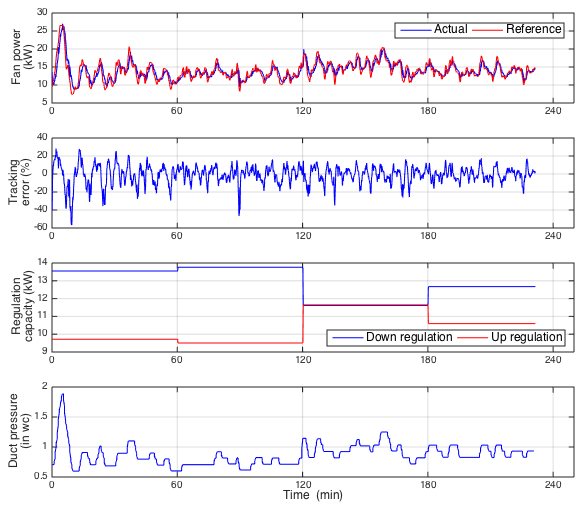
\includegraphics[width=\textwidth]{chapters/building_exp/figures/Track_power.png}
%\vspace*{-0.4cm}
\caption{Tracking experiment results: power, tracking error, regulation capacities and duct pressure.}
\label{fig:track_power}
%\vspace*{-0.45cm}
\end{figure}

\begin{figure}[t]
\centering
%\vspace*{-0.5cm}
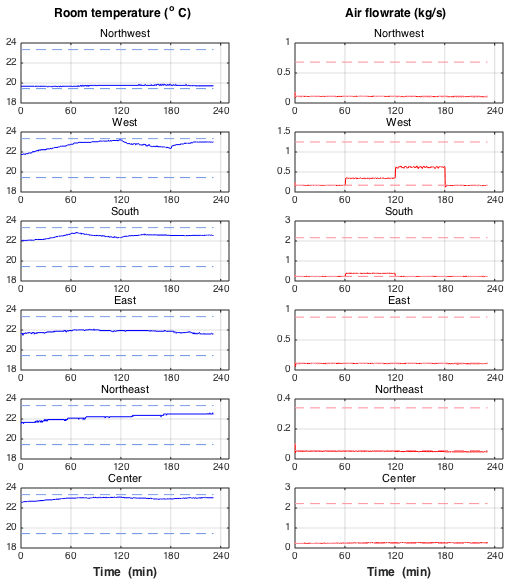
\includegraphics[width=\textwidth]{chapters/building_exp/figures/Track_temp_flow.png}
%\vspace*{-0.9cm}
\caption{Tracking experiment results: room temperatures and airflow rates. Solid lines are actual values, dashed lines are maximum and minimum limits.}
\label{fig:track_temp_flow}
%\vspace*{-0.45cm}
\end{figure}



%%%%%%%%%%%%%%%%%%%%%%%%%%%%%%%%%%%%%%%%%%%%%%%%%%%%
%%%%%%%%%%%%%%%%%%%%%%%%%%%%%%%%%%%%%%%%%%%%%%%%%%%%
%
%\subsection{Economic Potential}\label{sec:eco_potential}
%In this section, we use PJM's publicly available policy manuals \cite{PJM12} and market data \cite{PJM_signal_price} to estimate the revenue that SDH and similar buildings can obtain for offering regulation service.
%The fourth floor provided a regulation capacity of 23.3 kW during its operational hours. 
%%Assuming that each of the seven floors of SDH can provide the same capacity as the fourth floor does, then the entire building can provide 163 kW capacity for frequency regulation. 
%Assuming the building provides regulation service throughout the day, and receives an average reward of \$7.98/MWh, based on PJM's 2016 market data \cite{PJM_signal_price}, then its yearly revenue is estimated to be \$1,630.
%% Divided regulation payment of $15.96 by 2, as payment is for 1MWh of up and down capacity, i.e. +/- 1MWh of capacity (2 MWh total) gets paid $15.96 per hour.


%In this section, we use PJM's publicly available policy manuals \cite{PJM12} and market data \cite{PJM_signal_price} to estimate the revenue that SDH and similar buildings can obtain for offering regulation service.
%The fourth floor provided a regulation capacity of 23.3 kW during its operational hours. 
%Assuming that each of the seven floors of SDH can provide the same capacity as the fourth floor does, then the entire building can provide 163 kW capacity for frequency regulation. 
%Assuming SDH provides regulation service throughout the day, and receives an average reward of \$7.98/MWh, based on PJM's market data for July 2016 \cite{PJM_signal_price}, then its yearly revenue is estimated to be \$11,300.
%% Divided regulation payment of $15.96 by 2, as payment is for 1MWh of up and down capacity, i.e. +/- 1MWh of capacity (2 MWh total) gets paid $15.96 per hour.
%







% !TEX root = ../../thesis.tex
\subsection{Conclusions}\label{sec:conclusions}
In this chapter, we demonstrate experimentally that commercial buildings equipped with VAV HVAC systems can provide frequency regulation, by varying the power consumption of the supply fans.
To do so, we improve on existing frequency regulation control algorithms and propose a two-level control scheme that is suitable even for buildings subjected to larger disturbances and/or modeling uncertainties.
Then, we demonstrate our controller's performance through numerous field experiments conducted in an occupied commercial building, using archived PJM frequency regulation signals.





